\newpage
\section{Programm Umsetzung}
Das Programm wurde wie angegeben in 4 Threads eingeteilt.
\begin{itemize}
    \item Main-Thread
    \begin{itemize}
        \item Initialisierung der anderen Threads
        \item UART und Crypto Device Initialisierung 
        \item Validate Hardware Compatibility 
        \item alle 5 Sekunden ein Lebenszeichen von sich geben. 
    \end{itemize} 
    \item UART-IN-Thread
    \begin{itemize}
        \item Einlesen der UART 
        \item Statemachine Implementierung
    \end{itemize}
    \item UART-OUT-Thread
    \begin{itemize}
        \item Ausgabe der in die Queue geschriebenen Messages
    \end{itemize}
    \item PROCESS-Thread
    \begin{itemize}
        \item Verwaltung der Entschlüsselung 
    \end{itemize}
\end{itemize}
\subsection{Blockschaltbild}
\begin{figure}[!ht]
    \centering
    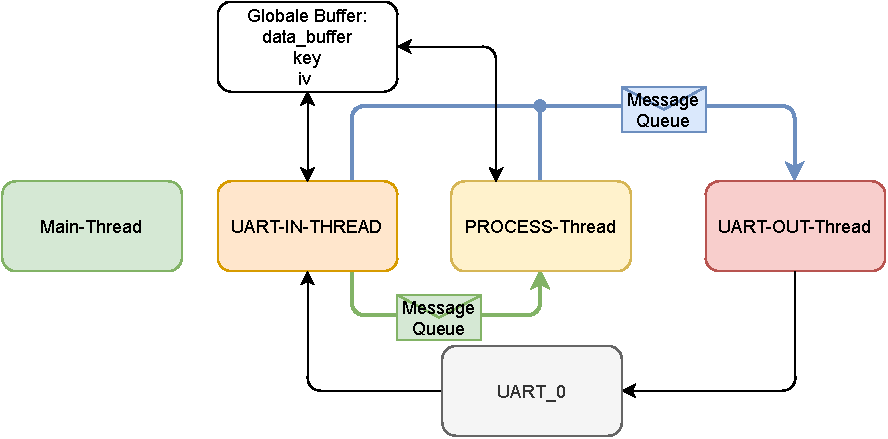
\includegraphics[width=\linewidth]{Blockschaltbild.pdf}
    \caption{Blockschaltbild}
    \label{fig:Blockschaltbild}
\end{figure}




\newpage
\subsection{Projekt Konfiguration}
Sodass, das nativ\_posix Board die benötigten Geräte verwenden kann müssen dieser in der \textbf{prj.conf} Datei aktivieren werden. 
\begin{lstlisting}[style=StyleC, captionpos=b, caption=prj.conf, label=pjr.conf]
#Configure Serial-Connection
CONFIG_SERIAL=y
CONFIG_UART_NATIVE_POSIX=y
CONFIG_NATIVE_UART_0_ON_OWN_PTY=y

#Configure Crypto
CONFIG_TINYCRYPT=y
CONFIG_TINYCRYPT_AES=y
CONFIG_TINYCRYPT_AES_CBC=y
CONFIG_CRYPTO=y
CONFIG_CRYPTO_TINYCRYPT_SHIM=y
\end{lstlisting}

\subsection{Initialisierung}
Es müssen:
\begin{itemize}
    \item Message-Queue 
    \item UART\_0 
    \item Verschlüsselung 
    \item Threads
\end{itemize}
initialisiert werden. 
    \subsubsection{Message-Queue}
        Wie in der Zephyr Dokumentation\footnote{\url{https://docs.zephyrproject.org/2.3.0/reference/kernel/data_passing/message_queues.html?highlight=queue}} beschrieben wird, kann eine 
        Message-Queue mit einem Macro initialisiert werden. 
        Für den Kryptoprozessor werden zwei Message-Queues verwendet, eine um die Nachrichten an der UART auszugeben und eine weitere um Befehle an den Process-Thread weiterzugeben. 
        \begin{lstlisting}[style=StyleC, captionpos=b, caption=Message-Queue-Initialisierung, label=Message-Queue-Initialisierung]
K_MSGQ_DEFINE(uart_queue, sizeof(struct uart_message *), q_max_msgs, q_align);
K_MSGQ_DEFINE(crypto_queue, sizeof(char* ), q_max_msgs, q_align);
        \end{lstlisting}



    \subsubsection{UART\_0}
    Um die UART verwenden zu können muss zuerst ein Device \anfuehrung{erstellt} werden. Dieses Gerät muss dan zur richtigen UART\_0 \textit{gebinded}/verbunden werden. 
    Danach kann die UART wie in der Dokumentation\footnote{\url{https://docs.zephyrproject.org/2.3.0/reference/peripherals/uart.html}} beschrieben konfiguriert werden. Da die UART in diesem Fall nur mit Pseudo-Terminal verwendet wird, ist die Konfiguration der Baudrate etc. nicht notwendig. 
    \begin{lstlisting}[style=StyleC, captionpos=b, caption=UART-Initialisierung, label=UART-Initialisierung]
const struct device * uart_dev; 
uart_dev = device_get_binding(UART_NAME);
if(!uart_dev){
    printk("UART-binding-error\n");
}
const struct uart_config uart_cfg = {
    .baudrate = 115200,
    .parity = UART_CFG_PARITY_NONE,
    .stop_bits = UART_CFG_STOP_BITS_1,
    .data_bits = UART_CFG_DATA_BITS_8,
    .flow_ctrl = UART_CFG_FLOW_CTRL_NONE
};

if(!uart_configure(uart_dev, &uart_cfg)){
    printk("UART-config-error\n");
}
        \end{lstlisting}

\newpage
    \subsubsection{Verschlüsselung}
        Die Initialisierung der Verschlüsselund bzw. des Crypto Device funktioniert sehr ähnlich wie bei der UART. Nur statt eine eigenen Konfiguration wird eine 
        Validate\_Hardware\_Funktion verwendet um zu Überprüfen wie das Crypto Device verwendet werden kann. Diese Funktion wurde vom CBC Beispiel von Zephyr kopiert. 
        \begin{lstlisting}[style=StyleC, captionpos=b, caption=UART-Initialisierung, label=UART-Initialisierung]
const struct device * crypto_dev;
static uint32_t cap_flags;

//bind crpyto
crypto_dev = device_get_binding(CRYPTO_DRV_NAME);
if (!crypto_dev) {
    printk("Crypto-binding-error\n");
    return;
}
//validate hardware for crypto device
validate_hw_compatibility();


int validate_hw_compatibility()
{
	uint32_t flags = 0U;
	flags = cipher_query_hwcaps(crypto_dev);
    if ((flags & CAP_RAW_KEY) == 0U) {
            printk("Please provision the key separately "
                    "as the module doesnt support a raw key\n");
            return -1;
    }

    if ((flags & CAP_SYNC_OPS) == 0U) {
            printk("The app assumes sync semantics. "
              "Please rewrite the app accordingly before proceeding\n");
            return -1;
    }

    if ((flags & CAP_SEPARATE_IO_BUFS) == 0U) {
            printk("The app assumes distinct IO buffers. "
            "Please rewrite the app accordingly before proceeding\n");
            return -1;
    }
	cap_flags = CAP_RAW_KEY | CAP_SYNC_OPS | CAP_SEPARATE_IO_BUFS;
	return 0;
}
        \end{lstlisting}


\newpage
    \subsubsection{Threads}
        Die Threads werden innerhalb des Main-Thread initialisiert. Dabei sind die Threads in einem Array und werden nacheinander gestartet. 
        \begin{lstlisting}[style=StyleC, captionpos=b, caption=UART-Initialisierung, label=UART-Initialisierung]
pthread_t thread_id[Number_of_threads];
init_threads(thread_id);
        
void init_threads(pthread_t* thread_id)
{	
	//init threads
	int i, thread_ok;
	void*(*threads[])(void*) = {uart_in_thread, uart_out_thread, process_thread};
	for(i=0; i<Number_of_threads; i++)
	{
		thread_ok = pthread_create(&thread_id[i], NULL, threads[i], NULL);
		if(thread_ok != 0)
		{
			printk("Thred creation Error\n");
		}
	}
}
        \end{lstlisting}


\subsection{UART-IN-Thread}
    Im UART-IN-Thread ist die Statemachine implementiert. Somit steuert dieser Thread alle Vorgänge im Prozessor. 
    Die States werden mittels einer Switch-Case abgefragt und gesetzt. 
    Um die States übersichtlich zu setzen wurde eine Enumeration verwendet. 
    \begin{lstlisting}[style=StyleC, captionpos=b, caption=Statemachine-Enumerations, label=Statemachine-Enumerations]
enum state{ INIT, ALIVE, AVAIL, KEY, IV, DECRYPT, DLEN, DATA, SELECT_OPERATION};
enum op{OP_KEY,OP_IV,OP_DECRYPT};
    \end{lstlisting}
    \begin{lstlisting}[style=StyleC, captionpos=b, caption=UART-IN-Thread, label=UART-IN-Thread]
void* uart_in_thread(void * x){
    state_machine();
    return x;
}
\end{lstlisting}
\newpage
    \begin{lstlisting}[style=StyleC, captionpos=b, caption=Statemachine, label=Statemachine, tabsize=1]
void state_machine()
{
    uint8_t i = 0;
    uint8_t uart_in;
    uint8_t* data_buffer = "";
    printk("In State Machine\n");
    while(1)
    {
        switch(st_state){
            case INIT: 
                if(!uart_poll_in(uart_dev, &uart_in)){
                    switch(uart_in){
                        case 'w':
                        case 'W':
                            put_message_in_crypto_queue("W\n");
                            break;
                        ...
                    }}
                break; 
            ...
            Pseudo-Code
            case DECRYPT
            //set busy flag, set op=OP_KEY, goto DLEN 
            case IV 
            //allocate data_buffer, set op=OP_IV, goto DATA
            case KEY 
            //allocate data_buffer, set op=OP_KEY, goto DATA
            case DLEN 
            //allocate data_buffer for data + iv, copy iv into buffer, move pointer from buffer where data should start, goto data
            CASE DATA 
            //get data from uart and put it into data_buffer, goto SELECT_OPERATION
            case SELECT_OPERATION: 
                switch(operation)
                {
                    case OP_KEY: 
                    //copy key from data_buffer into global key variable, goto state = INIT
                    case OP_IV: 
                    //copy iv from data_buffer into global iv variable, goto state = INIT
                    case OP_DECRYPT
                    //reset pointer from data_buffer, copy data_buffer into a global buffer, goto state = INIT
                }
        }
    }
}
    \end{lstlisting}




\newpage
\subsection{UART-Out-Thread}
Der UART-OUT-Thread sendet die Daten, die in der UART-Message-Queue stehen. 
Da die Daten für die finalen Tests teilweise mit Nullterminierung geschickt werden müssen wurde für die UART-Message-Queue ein Struct 
erstellt um die länge der Message festzulegen, da \textit{strlen()} nur bis zur Nullterminierung zählt.
\begin{lstlisting}[style=StyleC, captionpos=b, caption=uart\_message-struct label=uart-message-struct]
struct uart_message{
    unsigned char* message; 
    uint32_t len; 
};
\end{lstlisting}
\begin{lstlisting}[style=StyleC, captionpos=b, caption=UART-OUT-Thread, label=UART-OUT-Thread]
//put string into uart queue
int put_message_in_uart_queue(unsigned char* str, uint32_t len)
{	
    static struct uart_message message; 
    message.message = str; 
    message.len = len;
    struct uart_message * message_pointer = &message;
    
    if(k_msgq_put(&uart_queue, &message_pointer, K_FOREVER)!=0){
        printk("Couldn't put message in queue!!\n");
    }
    return 0;
}    
//send uart messages from queue
void* uart_out_thread(void * x)
{
	int i=0;
	uint32_t len; 
	struct uart_message * message;
	unsigned char* message_temp;
	while(1)
	{
		if(!k_msgq_get(&uart_queue, &message, K_NO_WAIT)) {
			len = message->len;
			message_temp = message->message; 
			while(i < len)
			{
				uart_poll_out(uart_dev, message_temp[i++]);
			}
			i = 0;
		}
	}
	return x;
}        
\end{lstlisting}


\newpage
\subsection{Processing Thread}
    Der Processing-Thread started die Entschlüsselung und verwaltet, wie in der Angabe beschrieben, das Senden vom "Processing-Available" und Blocken des Threads.
    \begin{lstlisting}[style=StyleC, captionpos=b, caption=Processing-Thread, label=Processing-Thread]
void * process_thread(void * x) 
{
    unsigned char* message;
    while(1)
    {
        if(!k_msgq_get(&crypto_queue, &message, K_NO_WAIT)) {
            
            switch (message[0])
            {
            case 'D':
                processing_busy = true; 
                if(cbc_mode())
                {
                    format_plaintext_for_comparison(out_buffer);
                }
                processing_busy = false;
                break;
            case 'P':
                processing_busy = true;
                put_message_in_uart_queue("PROCESSING AVAILABLE\n", strlen("PROCESSING AVAILABLE\n"));
                processing_busy = false;
                break; 
            case 'W':
                processing_busy = true; 
                sleep(10);
                processing_busy = false; 
                break; 
            
            
            default:
                break;
            }
        }
    }
    return x;
}        
    \end{lstlisting}


\newpage
\subsubsection{Entschlüsselung}
Für die Entschlüsselung sind standard IV und Key und ein Input und Output Buffer nötig. Diese werden global und in der Statemachine entsprechend der Angabe gesetzt. 
\begin{lstlisting}[style=StyleC, captionpos=b, caption=UART-Initialisierung, label=UART-Initialisierung]
//set default ciphertext BBBBBBBBBBBBBBBB
static uint8_t iv[AES_IV_LEN] ={
    0x42,0x42,0x42,0x42,
    0x42,0x42,0x42,0x42,
    0x42,0x42,0x42,0x42,
    0x42,0x42,0x42,0x42,
};
//set default key, with care so that iv and key are not overwriting each other
uint8_t* key = iv;
static uint8_t* cbc_buffer;
static uint8_t* out_buffer;    

int cbc_mode()
{	
	uint32_t  in_buffer_len = len + AES_IV_LEN; 
	uint32_t out_buffer_len = len; 
	out_buffer = malloc(out_buffer_len);
	struct cipher_ctx ini = {
		.keylen = AES_KEY_LEN,
		.key.bit_stream = key,
		.flags = cap_flags,
	};
	struct cipher_pkt decrypt = {
		.in_buf = cbc_buffer,
		.in_len = in_buffer_len,
		.out_buf = out_buffer,
		.out_buf_max = out_buffer_len,
	};
	if(cipher_begin_session(crypto_dev, &ini, CRYPTO_CIPHER_ALGO_AES, CRYPTO_CIPHER_MODE_CBC, CRYPTO_CIPHER_OP_DECRYPT)){
		cipher_free_session(crypto_dev, &ini); put_message_in_uart_queue("XERROR\n", strlen("XERROR\n")); return 0;
	} 
	if (cipher_cbc_op(&ini, &decrypt, cbc_buffer)) {
		cipher_free_session(crypto_dev, &ini); put_message_in_uart_queue("XERROR\n", strlen("XERROR\n")); return 0;
	}
	cipher_free_session(crypto_dev, &ini);
	return 1;
}
\end{lstlisting}


\newpage
\subsection{Test-Ausführung}
\begin{figure}[!htb]
    \centering
    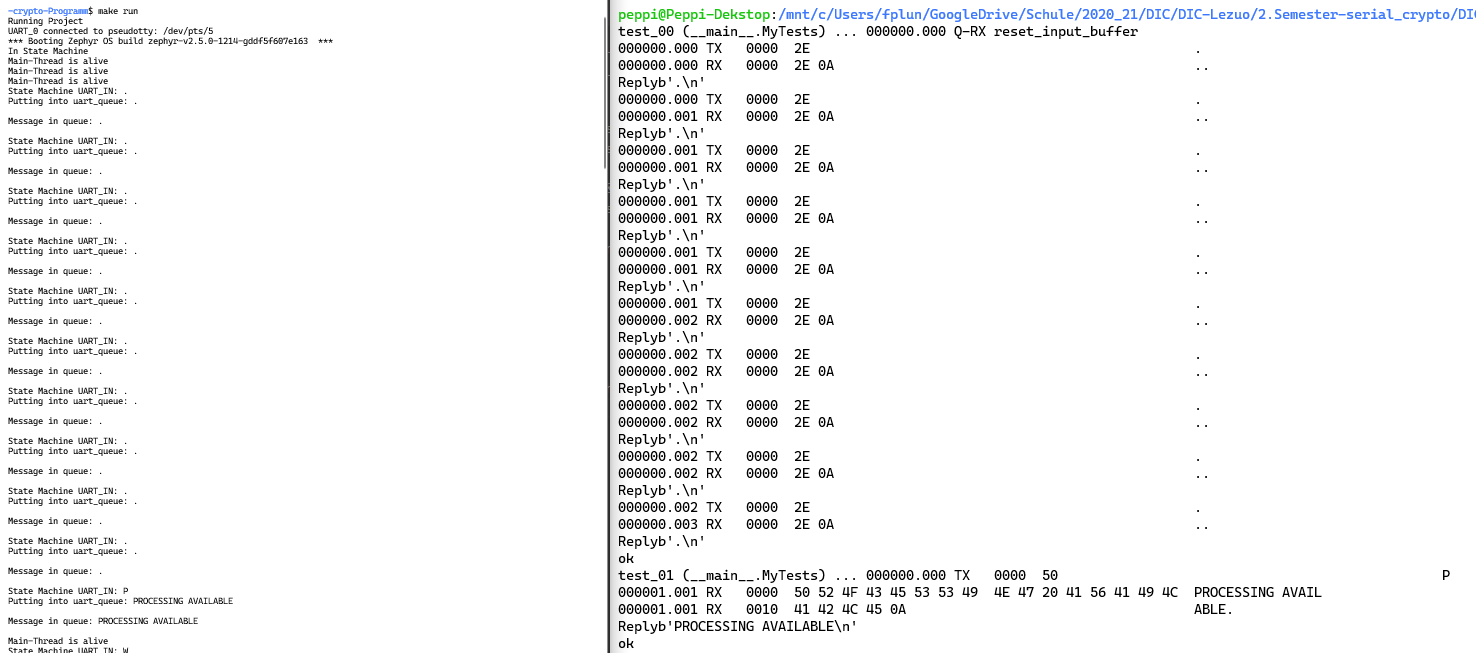
\includegraphics[width=\linewidth]{Test00-01.png}
    \caption{Test00-01}
    \label{caption:Test00-01}
\end{figure}
\begin{figure}[!htb]
    \centering
    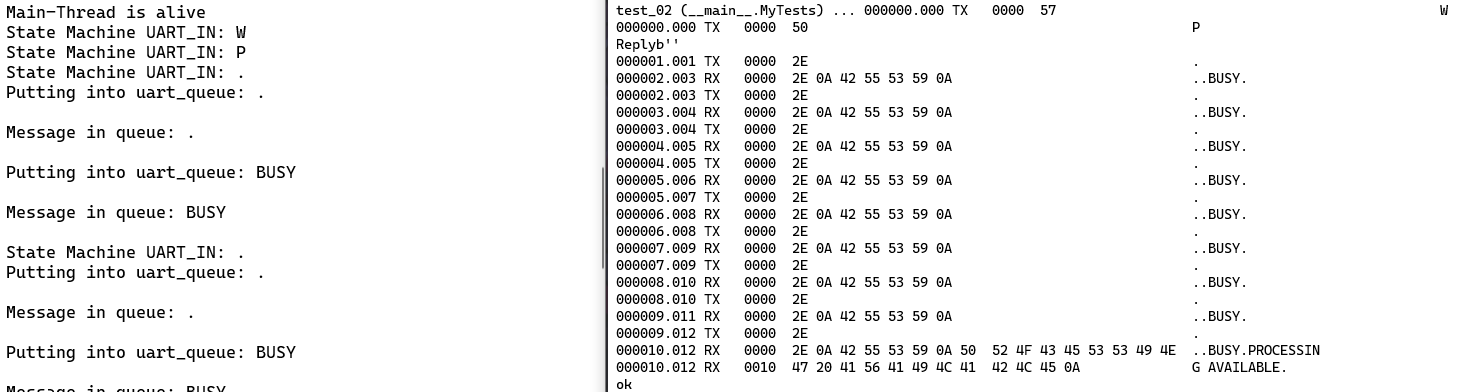
\includegraphics[width=\linewidth]{Test02.png}
    \caption{Test02}
    \label{caption:Test02}
\end{figure}
\begin{figure}[!htb]
    \centering
    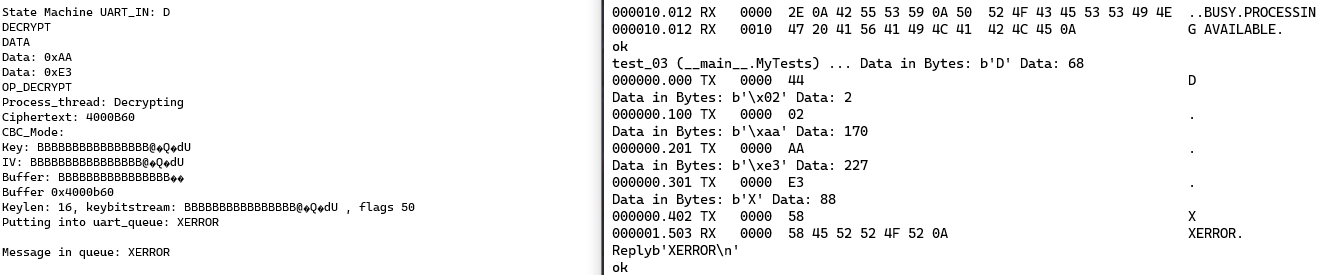
\includegraphics[width=\linewidth]{Test03.png}
    \caption{Test03}
    \label{caption:Test03}
\end{figure}
\begin{figure}[!htb]
    \centering
    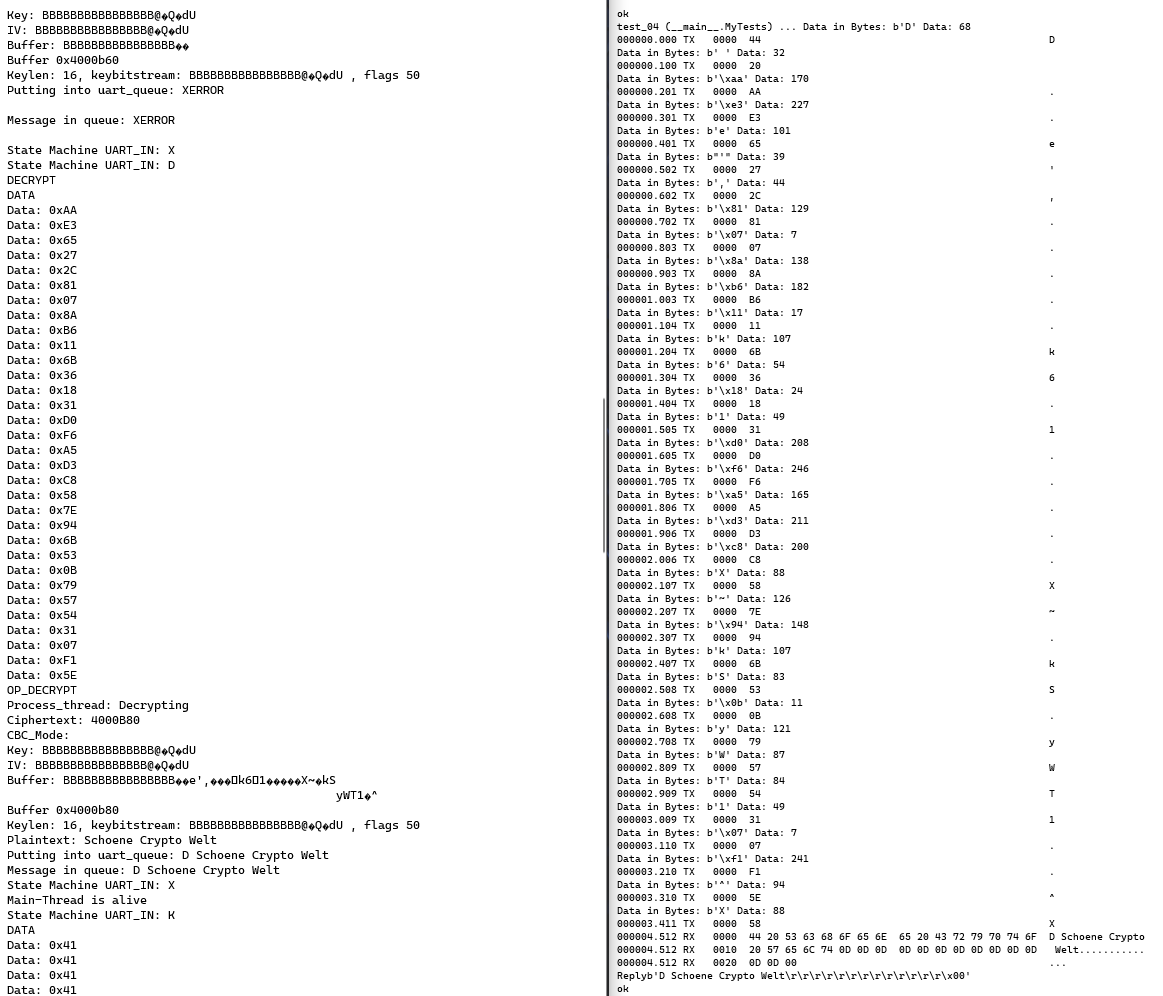
\includegraphics[width=\linewidth]{Test04.png}
    \caption{Test04}
    \label{caption:Test04}
\end{figure}
\begin{figure}[!htb]
    \centering
    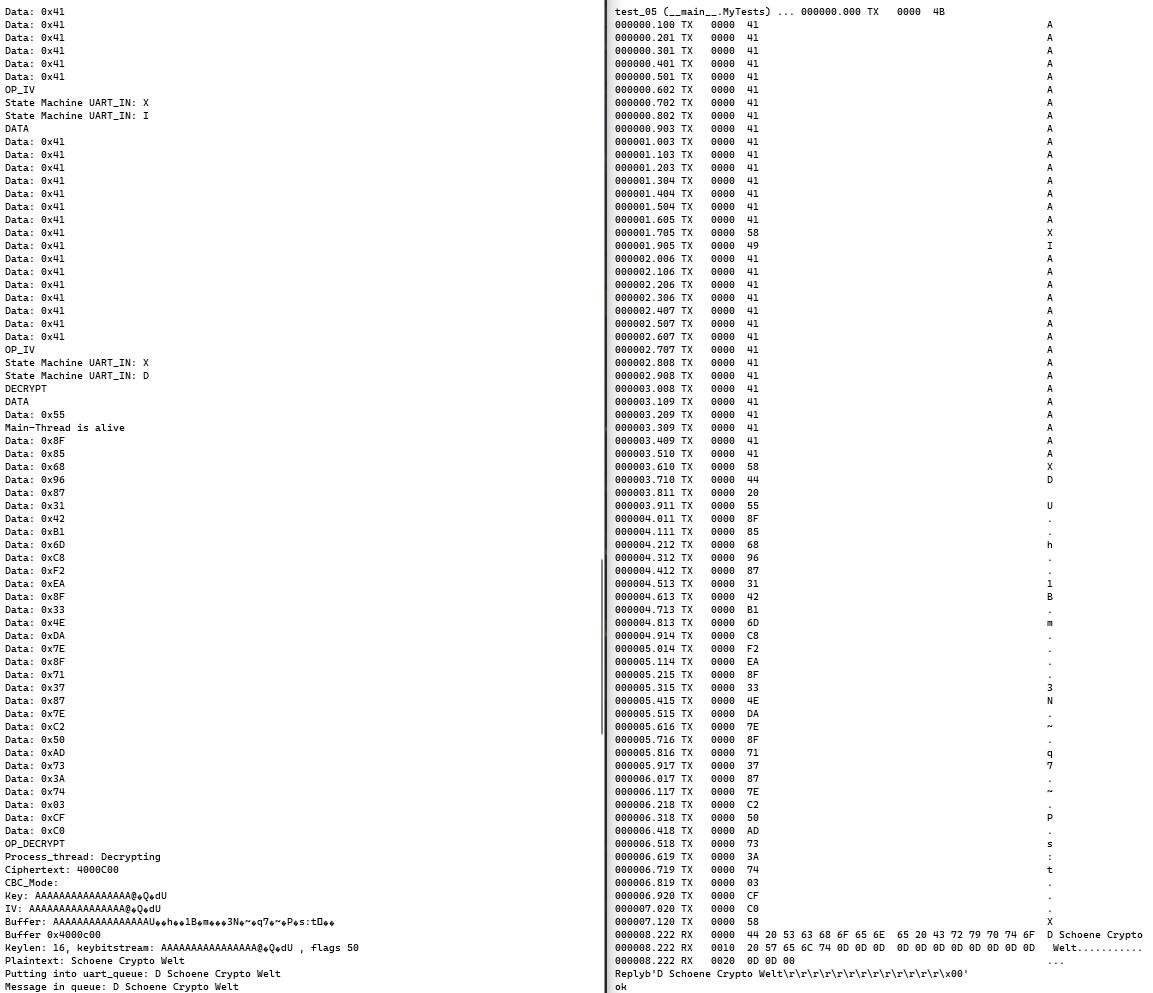
\includegraphics[width=\linewidth]{Test05.png}
    \caption{Test05}
    \label{caption:Test05}
\end{figure}
